% =====================================================================
\chapter{Part B: Simulation Results}
\label{ch:partb-results}
\thispagestyle{plain}
% =====================================================================

\section{Introduction}

This chapter presents the closed-loop evaluation of the Part~B controllers. Section~\ref{sec:rb-protocol} first describes the traffic families, the reference controllers and the statistical protocol. The B1 results follow in Sections~\ref{sec:rb-main}--\ref{sec:rb-overhead}. They cover the main comparison, the source of the gain, the ablations, the 3GPP traffic family, robustness, the interaction with Part~A compression and the decision overhead. Section~\ref{sec:rb-ext} then reports the extended study and Section~\ref{sec:rb-b2} the Bayesian Transformer forecaster. Section~\ref{sec:rb-b3} covers the back-pressure newsvendor, which is the final and best controller of the project.

\section{Evaluation Protocol}
\label{sec:rb-protocol}

\subsection{Traffic families}

We use three independent traffic families, so that no conclusion rests on a single traffic model:
\begin{itemize}
  \item \textbf{Family S (synthetic, bursty).} Gamma background traffic is combined with ON/OFF bursts whose sojourns are heavy-tailed Pareto ($\alpha_{\rm on} = 1.5$, $\alpha_{\rm off} = 1.8$)~\cite{willinger1997}, together with slow load regimes and drift in spectral efficiency. There are five scenarios: low (offered load 0.50), moderate (0.65), high (0.80), flash crowds, and a \textbf{held-out distribution shift} that is never seen in training or tuning.
  \item \textbf{Family G (standards-based, nothing hand-designed).} The geometry is 3GPP TR 38.901 UMa with 7 interfering sites and Jakes fading~\cite{tr38901}, and channel quality is mapped with the TS 38.214 CQI table~\cite{ts38214}. eMBB cells carry FTP Model~3 traffic~\cite{tr36814}, and LL cells carry XR video at 60~fps~\cite{tr38838}. The fronthaul demand is the output of a round-robin PRB scheduler. We run this family at moderate (0.65) and high (0.80) load.
  \item \textbf{Family M (Markov-modulated).} Gamma sources are modulated by a Markov chain with idle, normal and burst phases. The scenarios are moderate and high load, plus a semi-Markov held-out shift with Pareto sojourns.
\end{itemize}

\subsection{Reference controllers}

\begin{table}[H]
\caption{Controllers of the B1 comparison (all tuned on validation seeds).}
\label{tab:b-controllers}
\centering\small
\setlength{\tabcolsep}{4pt}
\begin{tabular}{lll}
\toprule
Controller & Estimate of $\rstar$ & Allocation \\
\midrule
Static equal & none & $C/N$ \\
Reactive proportional & mean-rate EWMA (deadline-unaware) & proportional water-fill \\
MaxWeight & priority $\times$ queue, HOL-age urgency & max-weight \\
Deadline-aware reactive & last observed $\rstar$ & deadline-weighted water-fill \\
Point forecast & GBM \textbf{median} & deadline-weighted water-fill \\
Fixed global quantile & GBM quantile, one tuned level (0.75) & water-fill \\
Proposed (window) & empirical quantiles, last 30 horizons (no ML) & KKT rule \\
\ours \textbf{Proposed} & \textbf{GBM quantiles} & \textbf{KKT rule} \\
Oracle water-fill & true $\rstar$ (reference only) & water-fill \\
Oracle + KKT & true $\rstar$ (reference only) & KKT rule \\
\bottomrule
\end{tabular}
\end{table}

Table~\ref{tab:b-controllers} lists the controllers of the B1 comparison. The point forecast is the most important ablation, since it uses the same model but passes on only one number. The fixed global quantile is included to check that simply reserving a high quantile is not what makes the method work. For every baseline we tuned the margins $\{0, 0.25, 0.5\}$, the EWMA windows and the persistence windows on validation seeds, and a margin of 0 turned out best for all of them. All baselines redistribute unused capacity and share the weights, backlog rate and water-fill of the point-forecast controller. The oracles use the true future $\rstar$ and serve only as references. The extended study adds predictive MaxWeight, the CEM policy, a model-based Markov-chain KKT rule, a bound-quantile KKT rule and a tuned-weight KKT rule, which brings the total to 19 controllers.

\subsection{Statistical protocol}

Each scenario is run for 20 test seeds of 20{,}000 slots (10~s), after 1{,}000 warm-up slots. All controllers receive the same traces and the same stale observations. The train, validation and test seeds do not overlap, and every forecaster is frozen before testing starts. Most of the variation from seed to seed comes from burst timing, which all controllers share, so we report paired per-seed comparisons. For each pair we give the mean relative change of $V_w$ with a 95\,\% bootstrap confidence interval, the number of seeds won out of 20, and a Wilcoxon signed-rank test with Holm correction. The simulation parameters are collected in Table~\ref{tab:b-params}.

\begin{table}[H]
\caption{Part~B simulation parameters.}
\label{tab:b-params}
\centering\small
\begin{tabular}{ll}
\toprule
Parameter & Value \\
\midrule
Cells & 8: 3 LL ($D = 2$~ms, $w = 3$), 5 eMBB ($D = 10$~ms, $w = 1$) \\
Link & 25GE, 3\,\% reserved $\Rightarrow C = 12.125$~Mbit per 0.5~ms slot \\
Over-subscription & $\sum_i$ peak$_i = 2.44\,C$ \\
Per-cell peak & 273 PRBs $\times$ 4 layers $\times\ \beta(9)$ $\approx$ 7.4~Gbit/s \\
Control interval, delay & $T = 20$ slots (10~ms), $\tau = 2$ slots (1~ms) \\
Forecast quantiles & 0.05, 0.25, 0.5, 0.75, 0.9, 0.95 \\
Seeds & train 1000--1015, validation 2000--2003, test 3000--3019 \\
Test length & 20 seeds $\times$ 20{,}000 slots after 1{,}000 warm-up \\
Statistics & paired bootstrap 95\,\% CI, Holm-corrected Wilcoxon \\
\bottomrule
\end{tabular}
\end{table}

\section{B1: Main Result on Family S}
\label{sec:rb-main}

Table~\ref{tab:b-main} lists $V_w$ for every controller in every scenario. Among the implementable controllers, the proposed KKT rule is best in all five scenarios, and this includes flash crowds and the held-out shift. At high load it reaches 8.00\,\%. The point forecast gives 9.70\,\% at the same load, reactive proportional 9.20\,\% and MaxWeight 11.54\,\%. Figure~\ref{fig:b-main} plots the same data.

\begin{table}[H]
\caption{B1 main result, Family S: $V_w$ [\%] (mean $\pm$ std over 20 test seeds; lower is better).}
\label{tab:b-main}
\centering\scriptsize
\setlength{\tabcolsep}{3.5pt}
\begin{tabular}{lccccc}
\toprule
Method & low 0.50 & moderate 0.65 & high 0.80 & flash crowds & shift (held-out) \\
\midrule
Static equal share & 4.45 $\pm$ 1.05 & 9.65 $\pm$ 1.36 & 15.46 $\pm$ 1.51 & 19.15 $\pm$ 2.34 & 22.31 $\pm$ 2.99 \\
Reactive proportional & 0.83 $\pm$ 0.27 & 4.11 $\pm$ 0.69 & 9.20 $\pm$ 0.99 & 12.27 $\pm$ 2.23 & 11.70 $\pm$ 2.24 \\
MaxWeight & 0.90 $\pm$ 0.28 & 4.85 $\pm$ 0.79 & 11.54 $\pm$ 1.27 & 15.24 $\pm$ 3.02 & 12.31 $\pm$ 2.44 \\
Deadline-aware reactive & 0.52 $\pm$ 0.21 & 4.24 $\pm$ 0.78 & 11.03 $\pm$ 1.33 & 14.51 $\pm$ 3.06 & 12.56 $\pm$ 2.81 \\
Point forecast (GBM median) & 0.27 $\pm$ 0.17 & 3.23 $\pm$ 0.73 & 9.70 $\pm$ 1.34 & 13.33 $\pm$ 3.09 & 11.30 $\pm$ 2.81 \\
Fixed global quantile (0.75) & 0.34 $\pm$ 0.23 & 4.35 $\pm$ 1.02 & 11.76 $\pm$ 1.44 & 15.09 $\pm$ 3.17 & 12.85 $\pm$ 3.32 \\
Proposed, window quantiles (no ML) & 0.25 $\pm$ 0.13 & 2.57 $\pm$ 0.64 & 8.72 $\pm$ 1.34 & 12.67 $\pm$ 3.19 & 10.22 $\pm$ 2.88 \\
\ours \textbf{Proposed (GBM + KKT)} & \textbf{0.15 $\pm$ 0.13} & \textbf{2.15 $\pm$ 0.60} & \textbf{8.00 $\pm$ 1.27} & \textbf{11.76 $\pm$ 3.08} & \textbf{10.04 $\pm$ 2.71} \\
\midrule
\textcolor{gray}{Oracle water-fill (reference)} & \textcolor{gray}{0.07} & \textcolor{gray}{1.62} & \textcolor{gray}{6.89} & \textcolor{gray}{10.16} & \textcolor{gray}{6.69} \\
\bottomrule
\end{tabular}
\end{table}

\begin{figure}[H]
\centering
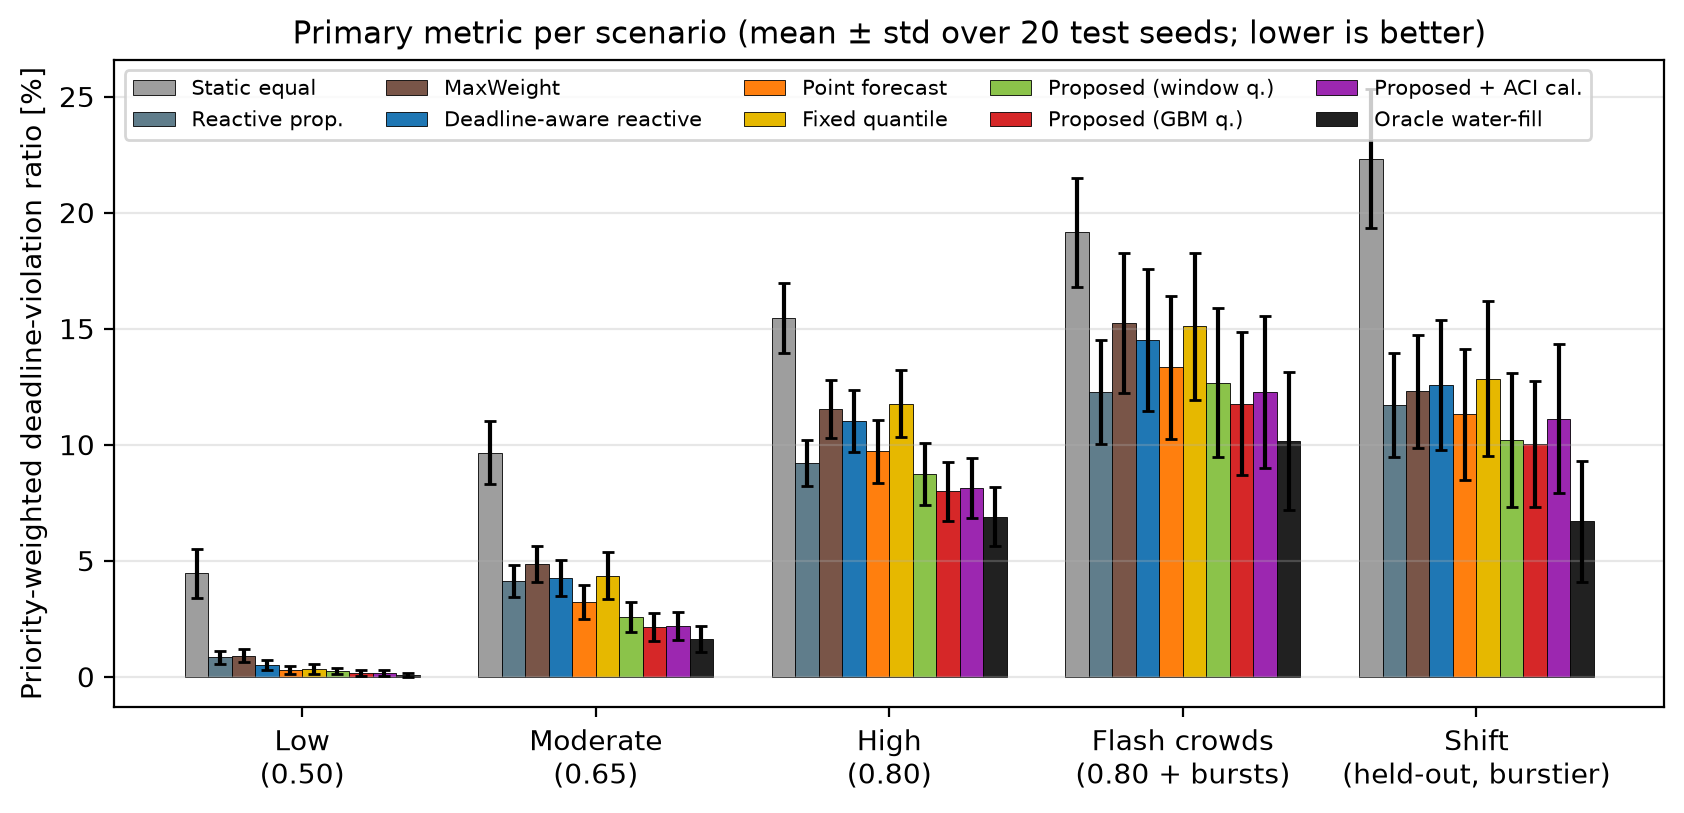
\includegraphics[width=0.9\textwidth]{fig1_primary_by_scenario.png}
\caption{Priority-weighted violation ratio by scenario, Family S; the proposed rule is lowest among implementable controllers everywhere.}
\label{fig:b-main}
\end{figure}

Table~\ref{tab:b-paired} gives the paired reductions per seed. We compared the proposed rule with the point forecast, the fixed quantile, MaxWeight and the deadline-aware reactive controller. It wins against each of them in every scenario, the held-out shift included, on all of the 20 seeds and with $p < 0.01$. Compared with the point forecast it has 11--43\,\% fewer weighted violations. The reduction is 22--54\,\% against the fixed quantile, 19--70\,\% against deadline-aware reactive and 18--83\,\% against MaxWeight. These reductions are plotted in Figure~\ref{fig:b-paired}.

\begin{table}[H]
\caption{Paired per-seed reduction of $V_w$ by the proposed rule, Family S (mean relative change, seeds won out of 20; ** Holm--Wilcoxon $p < 0.01$, * $p < 0.05$).}
\label{tab:b-paired}
\centering\scriptsize
\setlength{\tabcolsep}{4pt}
\begin{tabular}{lccccc}
\toprule
Proposed vs. & low & moderate & high & flash crowds & shift \\
\midrule
Reactive proportional & $-81$\,\% 20/20** & $-48$\,\% 20/20** & $-13$\,\% 20/20** & $-4$\,\% 16/20* & $-14$\,\% 20/20** \\
MaxWeight & $-83$\,\% 20/20** & $-56$\,\% 20/20** & $-31$\,\% 20/20** & $-23$\,\% 20/20** & $-18$\,\% 20/20** \\
Deadline-aware reactive & $-70$\,\% 20/20** & $-49$\,\% 20/20** & $-27$\,\% 20/20** & $-19$\,\% 20/20** & $-20$\,\% 20/20** \\
Point forecast & $-43$\,\% 20/20** & $-33$\,\% 20/20** & $-18$\,\% 20/20** & $-12$\,\% 20/20** & $-11$\,\% 20/20** \\
Fixed global quantile & $-54$\,\% 20/20** & $-50$\,\% 20/20** & $-32$\,\% 20/20** & $-22$\,\% 20/20** & $-22$\,\% 20/20** \\
Window quantiles (no ML) & $-37$\,\% 20/20** & $-16$\,\% 20/20** & $-8$\,\% 20/20** & $-7$\,\% 20/20** & $-2$\,\% 16/20** \\
\bottomrule
\end{tabular}
\end{table}

\begin{figure}[H]
\centering
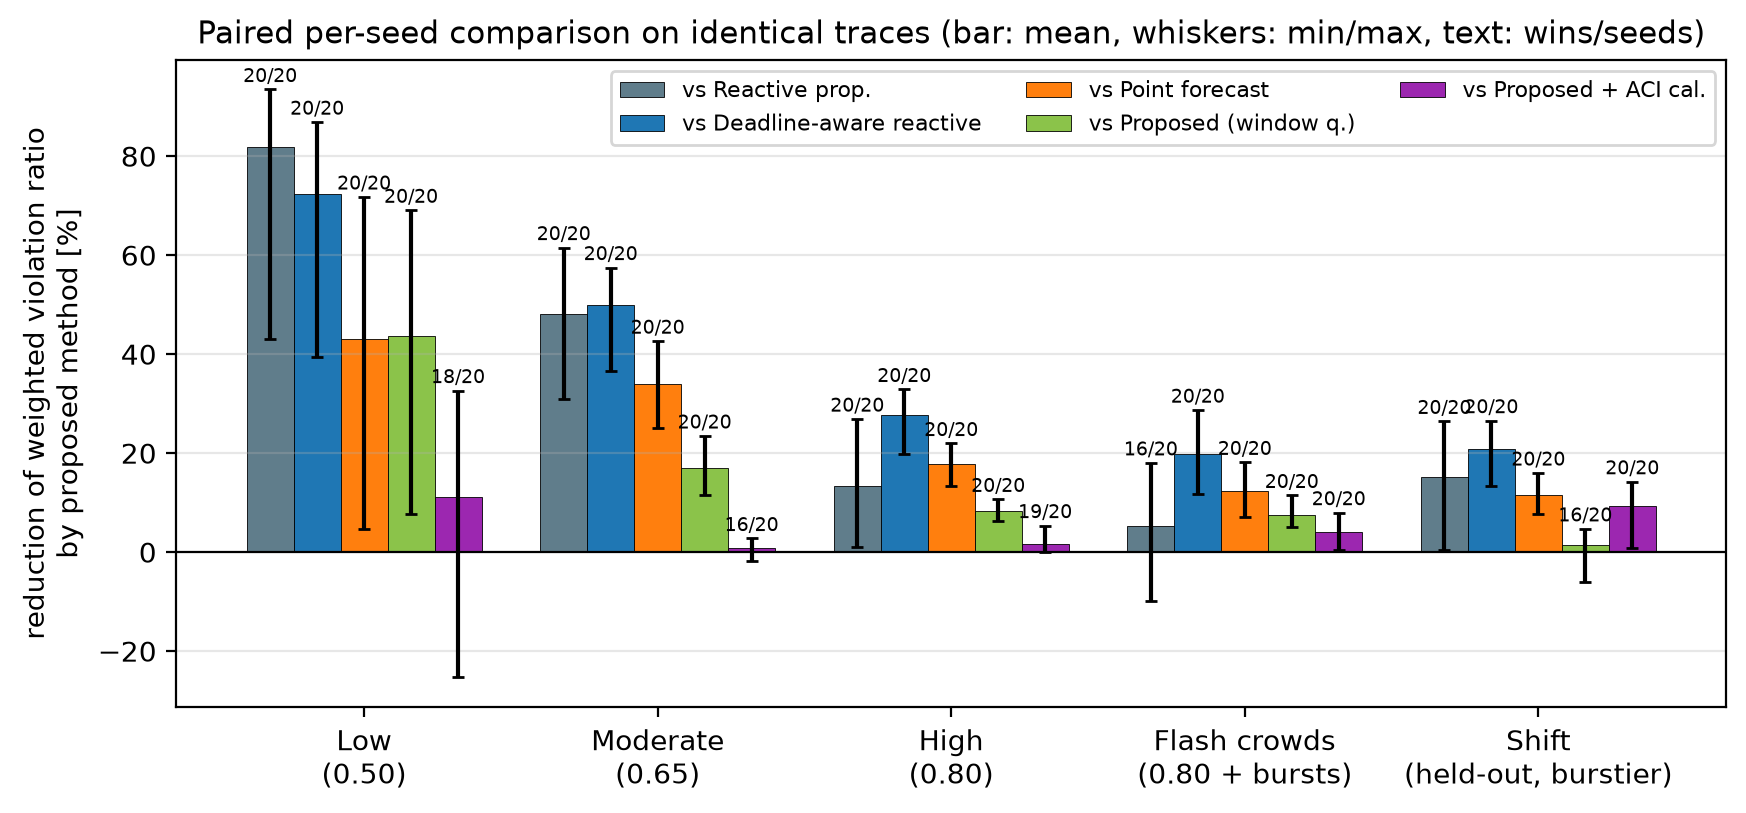
\includegraphics[width=0.85\textwidth]{fig8_paired_reduction.png}
\caption{Paired per-seed reductions of $V_w$ achieved by the proposed rule against each baseline.}
\label{fig:b-paired}
\end{figure}

\section{Where the Gain Comes From}
\label{sec:rb-where}

Table~\ref{tab:b-class} breaks down the high-load result for the deadline-aware controllers. The proposed rule has the lowest eMBB loss (12.3\,\%) and the highest link utilisation (72.2\,\%). This is because it adds margin only where the forecast is wide. A single global quantile level, in contrast, over-protects LL and wastes a third of its allocation. The proposed rule also has the highest Jain fairness (0.997).

\begin{table}[H]
\caption{Deadline-aware controllers, Family S, high load (20 seeds).}
\label{tab:b-class}
\centering\small
\begin{tabular}{lccc}
\toprule
Method & eMBB viol. & Utilisation & Jain \\
\midrule
Deadline-aware reactive & 16.5\,\% & 69.3\,\% & 0.995 \\
Point forecast & 16.0\,\% & 70.1\,\% & 0.994 \\
Fixed global quantile & 22.0\,\% & 67.0\,\% & 0.985 \\
\ours \textbf{Proposed} & \textbf{12.3\,\%} & \textbf{72.2\,\%} & \textbf{0.997} \\
\bottomrule
\end{tabular}
\end{table}

\begin{figure}[H]
\centering
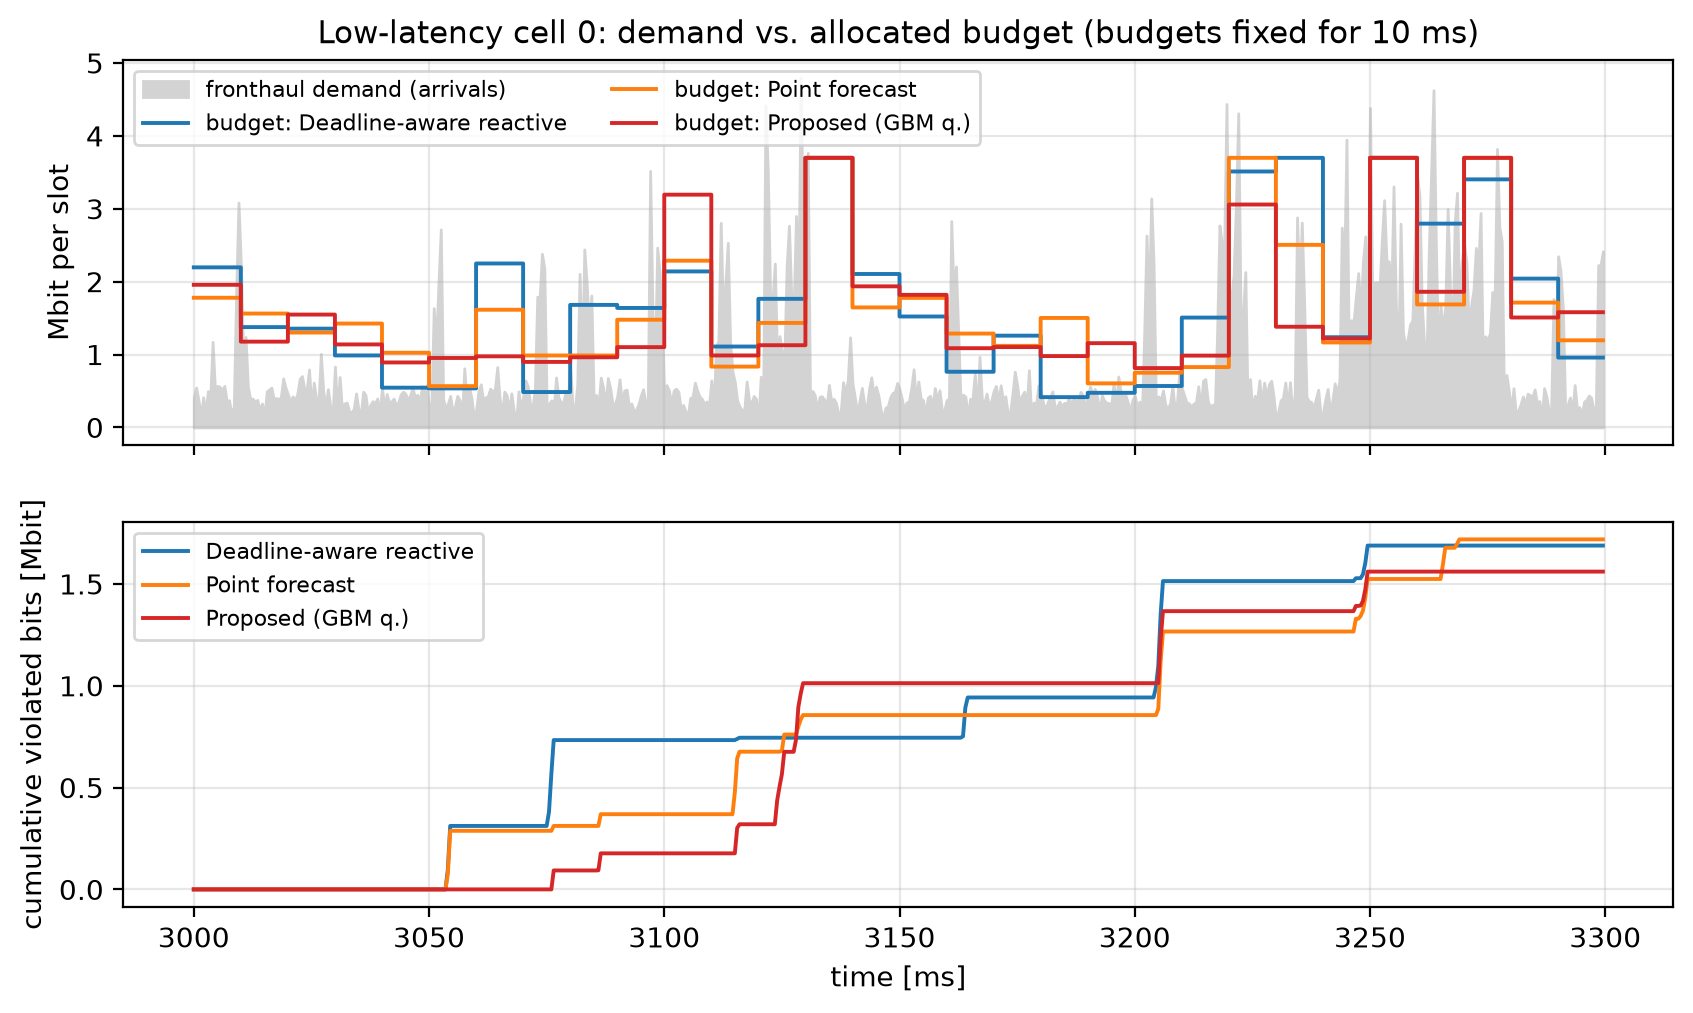
\includegraphics[width=0.7\textwidth]{fig6_demo_timeseries.png}
\caption{The rule in action on one LL cell: grey is demand, steps are budgets held for 10~ms. The reactive controller is one interval late at every burst, while the proposed rule raises the budget at burst onset, where the forecast range is wide, and accumulates the fewest violated bits.}
\label{fig:b-demo}
\end{figure}

\section{Ablations}
\label{sec:rb-abl}

Each ablation below changes one design choice and keeps everything else fixed:
\begin{enumerate}
  \item \textbf{A range versus a single number} (same model, same rule family): $-11$\,\% to $-43$\,\%, with 20/20 seeds in every scenario. This shows that \emph{representing uncertainty matters}.
  \item \textbf{Per-cell KKT level versus one tuned global level} (same forecast): $-22$\,\% to $-54$\,\%. So \emph{the level has to be set per cell by the link constraint}, which is what the KKT rule does.
  \item \textbf{GBM versus window (no-ML) quantiles} under the same KKT rule: GBM adds $-7$\,\% to $-37$\,\% on nominal traffic. Even the no-ML version beats the point forecast in every scenario. The rule itself therefore carries the method, and the learned forecaster improves on it further.
\end{enumerate}

\section{B1 on Family G: Standards-Based 3GPP Traffic}
\label{sec:rb-g}

Table~\ref{tab:b-g} and Figure~\ref{fig:b-g} show that the result carries over to traffic we did not design ourselves. The proposed rule is the best implementable controller at both loads, on 20/20 seeds. At high load it is 11\,\% better than the point forecast, 31\,\% better than deadline-aware reactive and 50\,\% better than reactive proportional. On this family our rule is also the best under the \emph{unweighted} violation ratio (14.3--14.4\,\% for the two variants). A forecaster trained on Family~S and used here without retraining still beats every reactive controller.

\begin{table}[H]
\caption{Family G (3GPP): $V_w$ [\%] at moderate and high load, and the unweighted ratio at high load.}
\label{tab:b-g}
\centering\small
\begin{tabular}{lccc}
\toprule
Method & moderate 0.65 & high 0.80 & unweighted (high) \\
\midrule
Static equal & 10.75 & 13.10 & 19.2 \\
Reactive proportional & 12.05 & 15.94 & 15.0 \\
MaxWeight & 17.51 & 25.79 & 19.7 \\
Deadline-aware reactive & 8.95 & 11.53 & 18.5 \\
Point forecast & 6.00 & 8.98 & 16.6 \\
Fixed quantile & 6.80 & 9.88 & 18.7 \\
Window quantiles & 6.18 & 9.01 & 16.0 \\
\ours \textbf{Proposed} & \textbf{5.08} & \textbf{8.01} & \textbf{14.4} \\
Transfer (trained on S) & 6.99 & 9.89 & 14.3 \\
\midrule
\textcolor{gray}{Oracle + KKT} & \textcolor{gray}{3.47} & \textcolor{gray}{6.06} & \textcolor{gray}{11.1} \\
\bottomrule
\end{tabular}
\end{table}

\begin{figure}[H]
\centering
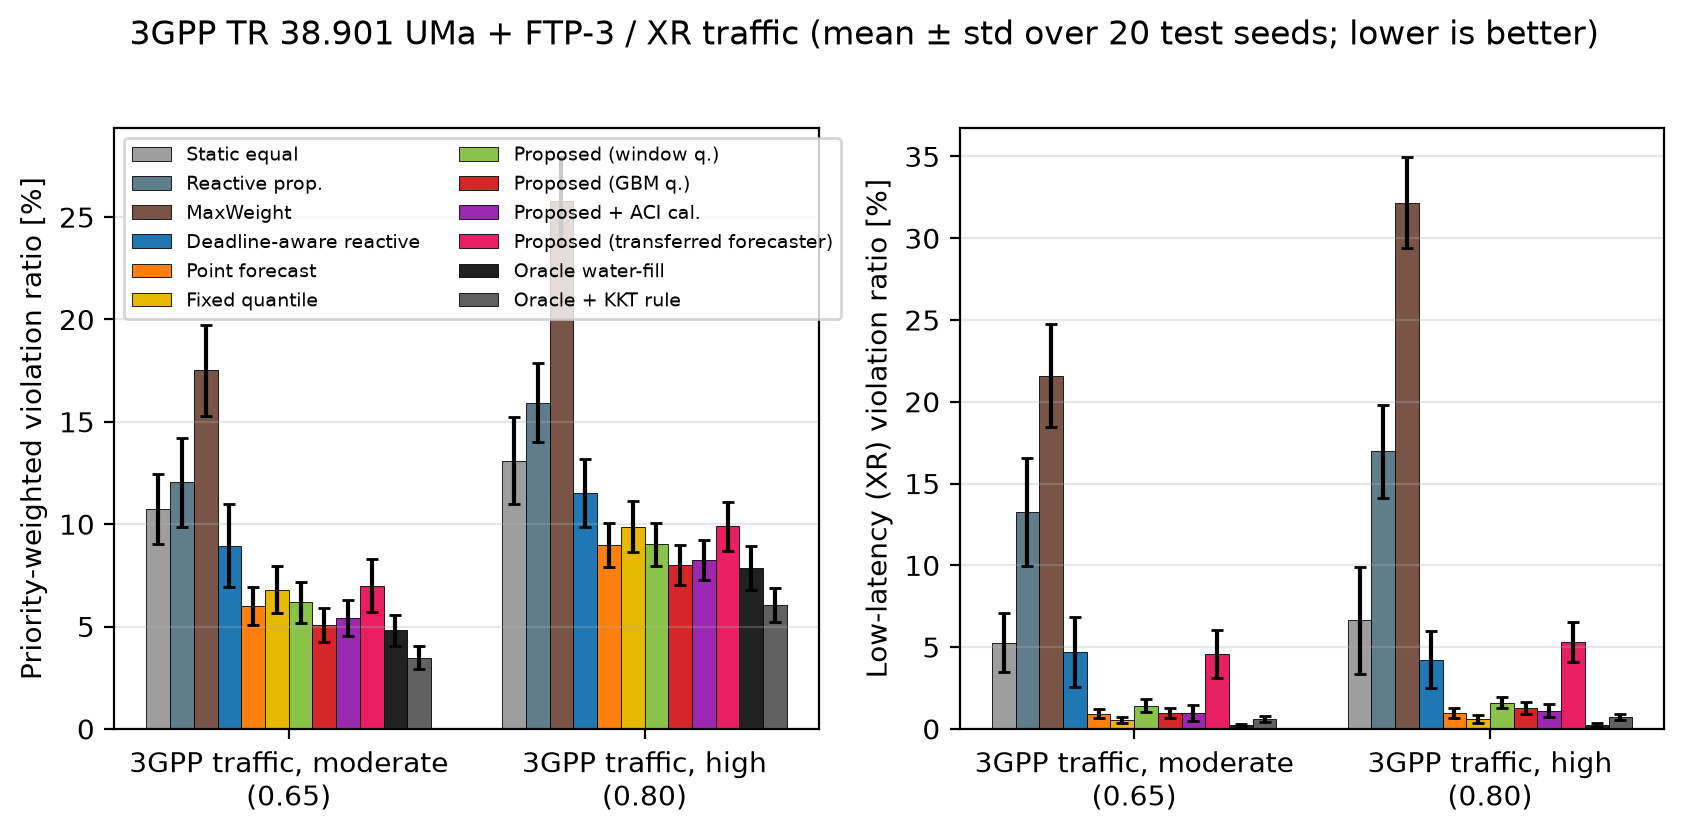
\includegraphics[width=0.8\textwidth]{fig12_tgpp.png}
\caption{Family G (3GPP UMa, FTP Model~3 and XR traffic): the proposed rule leads at both loads.}
\label{fig:b-g}
\end{figure}

\section{Forecast Quality, Robustness and Operating Regime}
\label{sec:rb-robust}

\paragraph{Forecast calibration.} On validation data the GBM quantiles cover 5.6 / 25.6 / 50.7 / 75.3 / 89.9 / 94.9\,\% at nominal levels 5 / 25 / 50 / 75 / 90 / 95\,\%, which means the forecaster is calibrated to within about one percentage point. Its pinball loss is 0.0224, compared with 0.0293 for a window median (Figure~\ref{fig:b-fq}).

\begin{figure}[H]
\centering
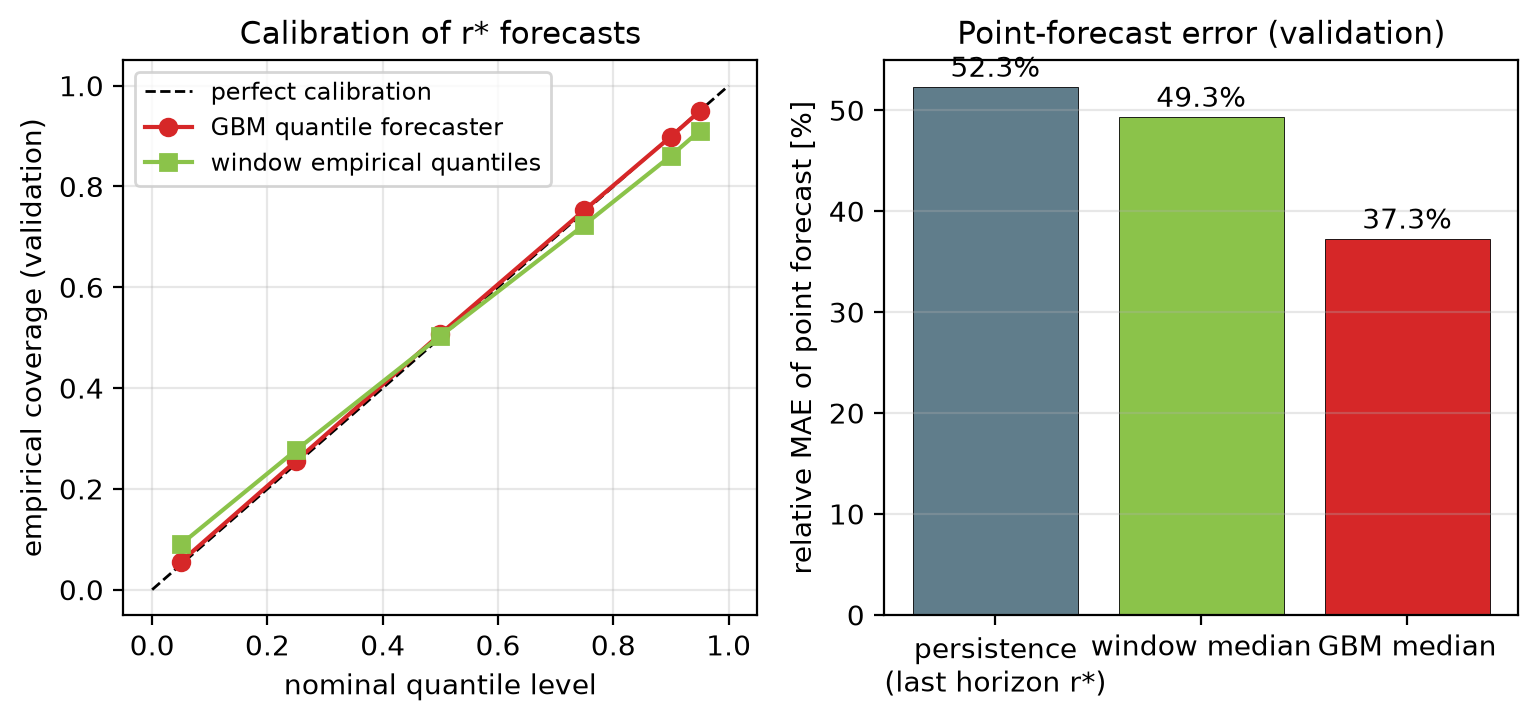
\includegraphics[width=0.62\textwidth]{fig5_forecast_quality.png}
\caption{Calibration of the GBM quantile forecaster on validation data.}
\label{fig:b-fq}
\end{figure}

\paragraph{Robustness to miscalibration.} To check Proposition~\ref{prop:robust} in practice, we shifted every forecast quantile level by $\epsilon$ before the allocation step (Table~\ref{tab:b-miscal}, Figure~\ref{fig:b-miscal}). Under-reserving does almost no harm, because the price $\lambda$ absorbs a common shift. Over-reserving makes things worse, but only gradually. Even at $\epsilon = 0.3$ the rule still matches the point forecast (9.46\,\%) and beats deadline-aware reactive (10.78\,\%).

\begin{table}[H]
\caption{$V_w$ [\%] when every quantile level is shifted by $\epsilon$ (10 seeds).}
\label{tab:b-miscal}
\centering
\begin{tabular}{lccccc}
\toprule
$\epsilon$ & $-0.3$ & $-0.1$ & 0 & $+0.1$ & $+0.3$ \\
\midrule
high & 7.80 & 7.61 & 7.71 & 8.13 & 9.45 \\
shift & 10.96 & 11.10 & 11.13 & 11.53 & 12.50 \\
\bottomrule
\end{tabular}
\end{table}

\begin{figure}[H]
\centering
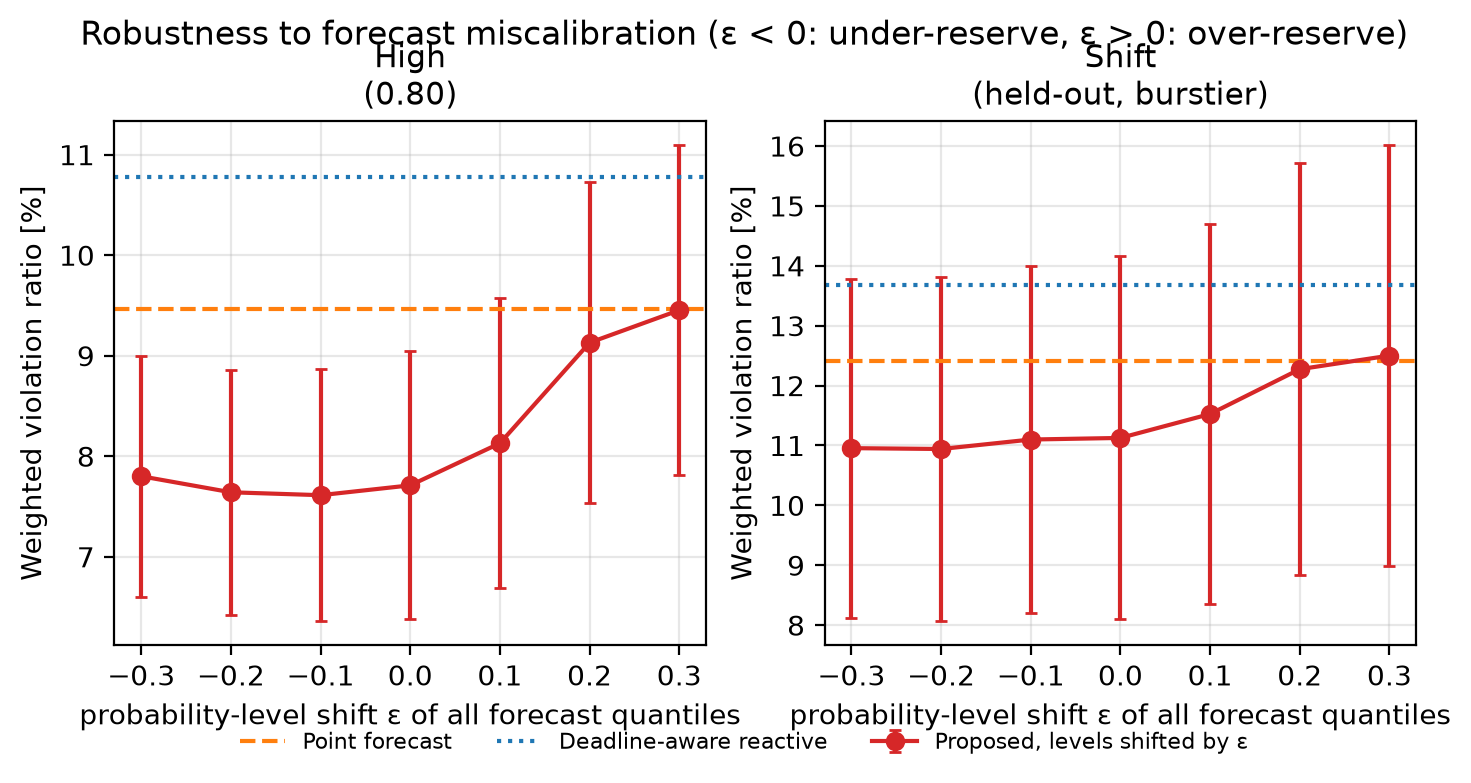
\includegraphics[width=0.6\textwidth]{fig10_miscalibration.png}
\caption{Robustness of the KKT rule to forecast miscalibration.}
\label{fig:b-miscal}
\end{figure}

\paragraph{Control interval and telemetry delay.} Table~\ref{tab:b-interval} varies the control interval and the telemetry delay (10 seeds). The KKT rule is the best controller for every interval from 2 to 10~ms, which is the operating range of a near-RT RIC. At $T = 2$~ms it even beats the oracle water-fill. The advantage is largest when telemetry is fresh ($-16$\,\% against reactive proportional at $\tau = 0$).

\begin{table}[H]
\caption{Sensitivity to control interval $T$ and telemetry delay $\tau$, Family S high load, $V_w$ [\%].}
\label{tab:b-interval}
\centering\small
\begin{tabular}{lccc}
\toprule
$T$ & Reactive prop. & Point forecast & \textbf{Proposed} \\
\midrule
2~ms & 3.91 & 6.57 & \textbf{3.07} \\
5~ms & 7.42 & 7.53 & \textbf{5.07} \\
10~ms & 8.91 & 9.46 & \textbf{7.71} \\
\midrule
$\tau$ & & & vs.\ reactive prop. \\
\midrule
0~ms & 8.16 & 8.45 & \textbf{6.85} ($-16$\,\%) \\
1~ms & 8.91 & 9.46 & \textbf{7.71} ($-13$\,\%) \\
2.5~ms & 9.86 & 10.51 & \textbf{8.77} ($-11$\,\%) \\
5~ms & 11.30 & 12.45 & \textbf{11.07} ($-2$\,\%) \\
\bottomrule
\end{tabular}
\end{table}

\paragraph{Priority weight.} The rule makes use of the operator's priority setting. When the LL weight is raised from 3 to 5, its $V_w$ at high load drops from 8.00 to 6.93\,\%, while that of reactive proportional grows from 9.20 to 10.56\,\%. So the more weight an operator puts on low-latency traffic, the larger the advantage of the proposed rule becomes.

\section{Part A $\times$ Part B: Compression Width and Allocation}
\label{sec:rb-ab}

The two parts of the project meet in the term $\beta(b)$ of Eq.~\eqref{eq:beta}. In Table~\ref{tab:b-ab} the user traffic is kept fixed and only the BFP width is changed. Compression determines the load regime, and allocation determines the loss within that regime. Moving from 9- to 6-bit mantissas lowers the load from 0.65 to 0.44. At 0.65 load the proposed rule cuts the loss of reactive proportional by half (1.96 vs 3.90\,\%). Part~A therefore keeps the link in the operating range where the Part~B allocation rule works best, and this is why the two parts belong together.

\begin{table}[H]
\caption{Compression width versus allocation rule (same user traffic), $V_w$ [\%].}
\label{tab:b-ab}
\centering
\begin{tabular}{lcccc}
\toprule
BFP width & offered load & Reactive prop. & Point forecast & \textbf{Proposed} \\
\midrule
6 bit & 0.44 & 0.22 & 0.15 & \textbf{0.11} \\
9 bit & 0.65 & 3.90 & 3.00 & \textbf{1.96} \\
\bottomrule
\end{tabular}
\end{table}


\section{Decision Overhead}
\label{sec:rb-overhead}

Figure~\ref{fig:b-time} shows the decision time per 10~ms epoch, measured in Python on a 4-core CPU. The KKT rule alone needs less than 0.1~ms. The complete proposed controller, which computes 28 features per cell and evaluates $6\times300$ trees, needs 3.5~ms. This is well inside the 10~ms interval. We also wrote a vectorised numpy tree traversal, and it runs 6.7$\times$ faster than scikit-learn's \texttt{predict} (1.8 vs 12~ms).

\begin{figure}[H]
\centering
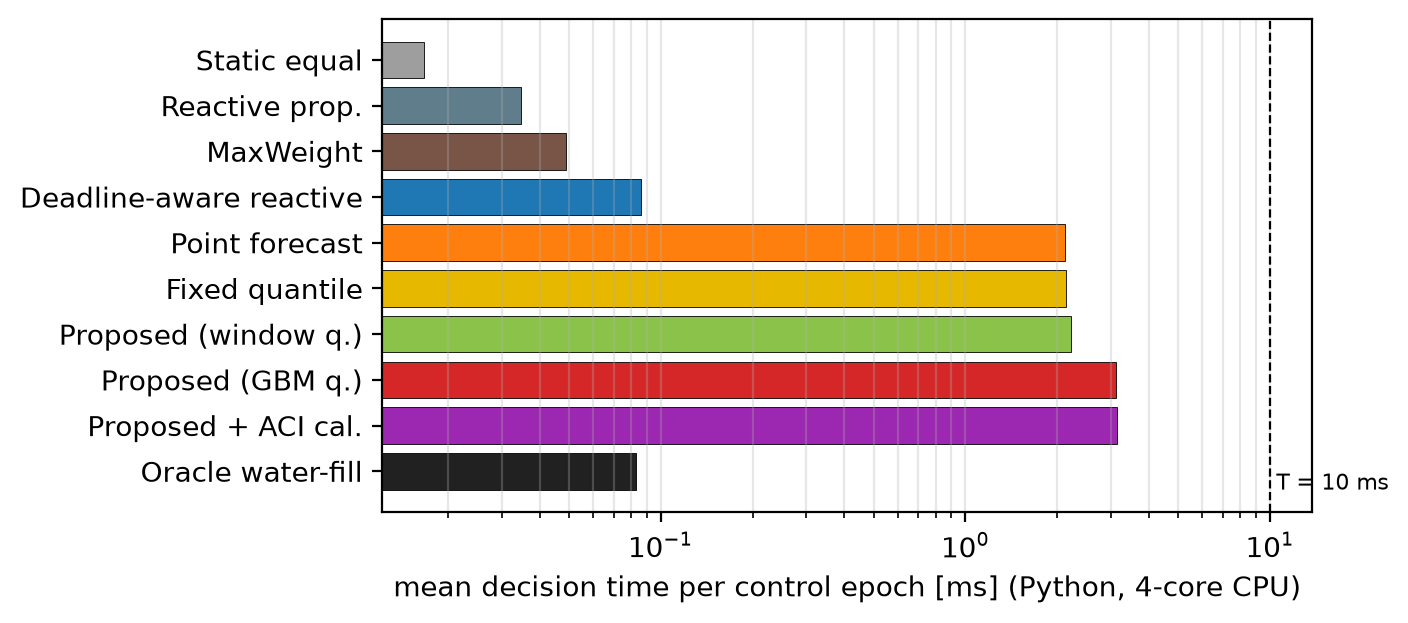
\includegraphics[width=0.62\textwidth]{fig7_decision_time.png}
\caption{Decision time per control epoch (Python, 4-core CPU).}
\label{fig:b-time}
\end{figure}

\section{Extended Study Results}
\label{sec:rb-ext}

Table~\ref{tab:b-ext} compares the best controllers of the extended study over all ten scenarios of the three families, and Figure~\ref{fig:b-ext} shows all 19 controllers. Within the NCC comparison set the KKT rule wins all 10 scenarios, and it is the best controller that has nothing to tune. A Markov chain fitted online, without any training data, comes within 3--9\,\% of the learned rule. Two controllers from the queueing and policy-search literature do better while using the \emph{same} forecaster. The CEM policy is best in 6 of 10 scenarios and predictive MaxWeight in 3, all of them on bursty Family~S. These two are the strongest baselines of the project, and B3 beats both of them.

\begin{table}[H]
\caption{Extended study: $V_w$ [\%] of the strongest controllers across three families.}
\label{tab:b-ext}
\centering\small
\setlength{\tabcolsep}{4pt}
\begin{tabular}{lccccc}
\toprule
Scenario & \makecell{GBM +\\KKT} & \makecell{Pred.\\MaxWeight} & \makecell{CEM\\policy} & \makecell{Markov-\\chain KKT} & \makecell{Tuned-$w$\\KKT} \\
\midrule
S low 0.50 & 0.15 & 0.14 & 0.13 & 0.25 & 0.18 \\
S moderate 0.65 & 2.15 & 1.62 & 1.77 & 2.65 & 2.21 \\
S high 0.80 & 8.00 & 6.15 & 6.57 & 8.64 & 7.88 \\
S flash crowd & 11.76 & 9.69 & 10.20 & 12.44 & 11.49 \\
S shift & 10.04 & 10.25 & 9.73 & 10.22 & 9.90 \\
G moderate 0.65 & 5.08 & 7.57 & 4.58 & 6.44 & 4.98 \\
G high 0.80 & 8.01 & 11.36 & 7.17 & 8.77 & 7.83 \\
M moderate 0.65 & 0.92 & 1.64 & 0.88 & 1.24 & 0.85 \\
M high 0.80 & 4.94 & 4.79 & 3.93 & 5.12 & 4.88 \\
M shift 0.80 & 5.52 & 4.80 & 4.17 & 5.39 & 5.31 \\
\bottomrule
\end{tabular}
\end{table}

\begin{figure}[H]
\centering
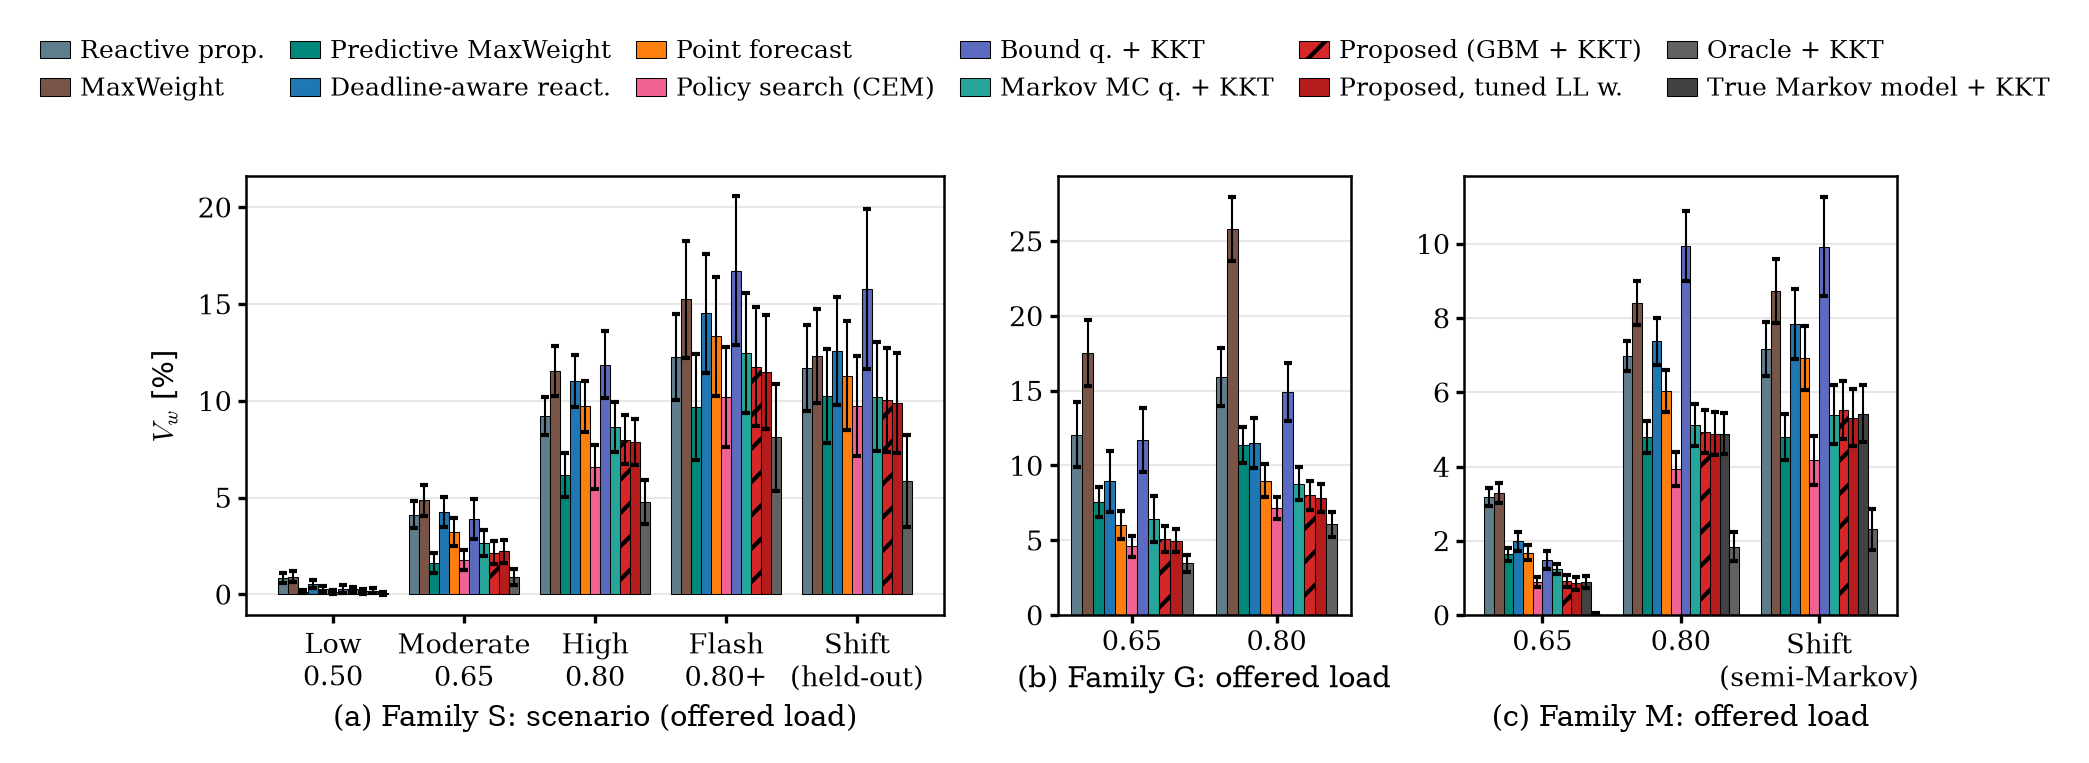
\includegraphics[width=\textwidth]{paper_fig_overview_ext.png}
\caption{All 19 controllers of the extended study on the three traffic families.}
\label{fig:b-ext}
\end{figure}

Looking at the KKT multiplier explains why the remaining gap has this shape. At high load the link is binding in 99.8--100\,\% of epochs, and $\lambda^\ast \ge w_{\rm eMBB}$ holds in 50--58\,\% of them. In half the epochs, then, every eMBB cell is already at its lowest quantile, and re-tuning the LL weight gains only 1--4\,\%. The CEM policy gains for a different reason, namely its \emph{decoupled} per-class levels and a different sharing rule. The gap comes from the structure of the rule and cannot be closed by changing a constant. Figure~\ref{fig:b-regime} maps out the operating regimes. Reservation wins for short intervals and for long bursts (FTP files, XR frames), while back-pressure wins for short bursts at 10--20~ms intervals. In Figure~\ref{fig:b-theory} the Markov-fluid theory is checked against simulation. The shortfall sandwich is never violated and the Chernoff bound holds.

\begin{figure}[H]
\centering
\begin{subfigure}{0.48\textwidth}
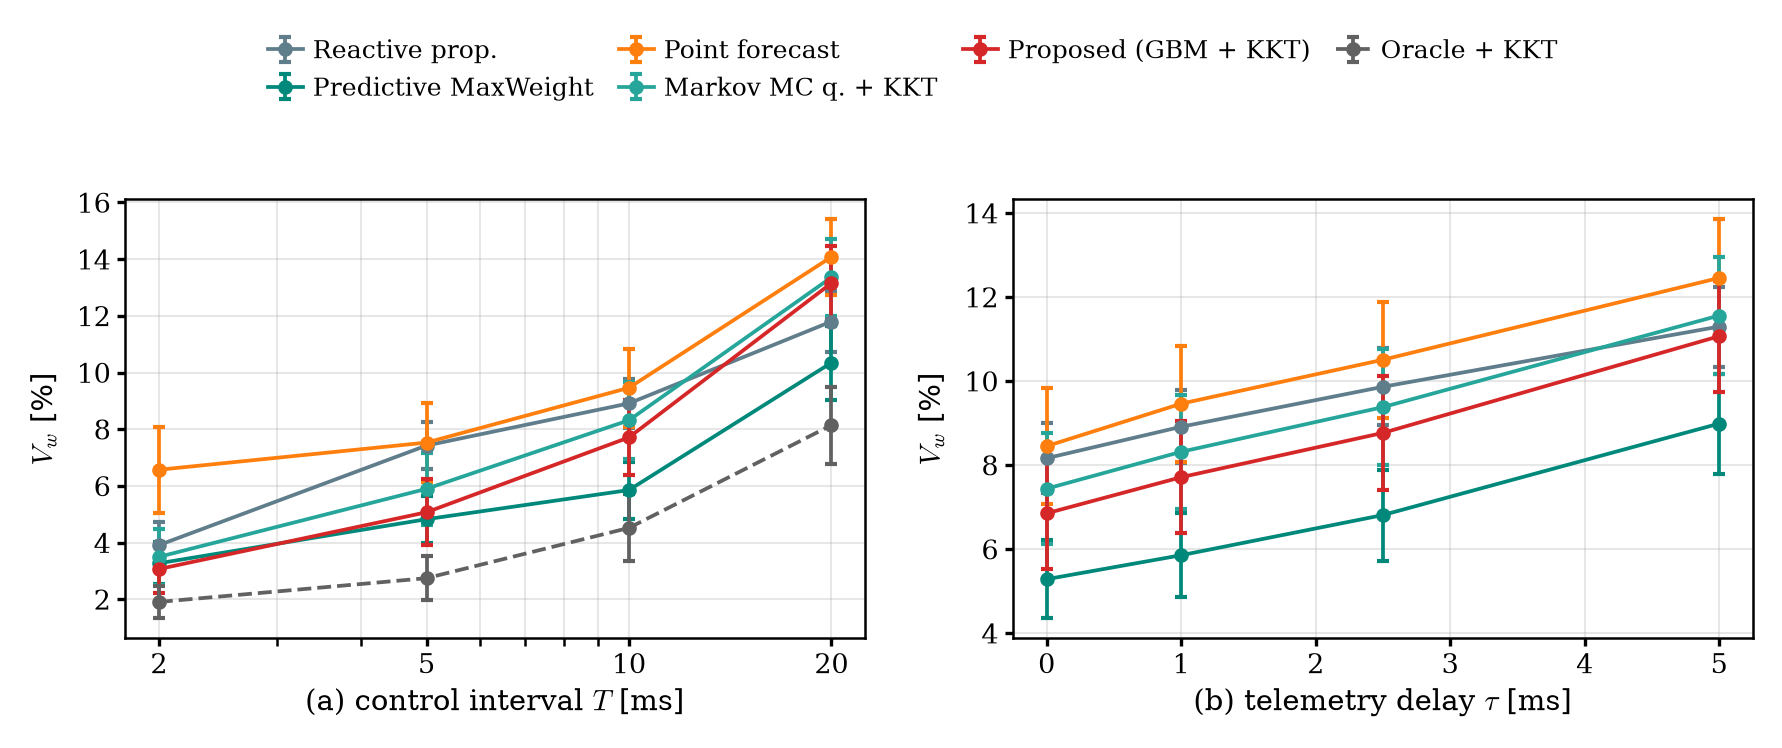
\includegraphics[width=\linewidth]{paper_fig_regime.png}
\caption{Operating regime.}
\label{fig:b-regime}
\end{subfigure}\hfill
\begin{subfigure}{0.5\textwidth}
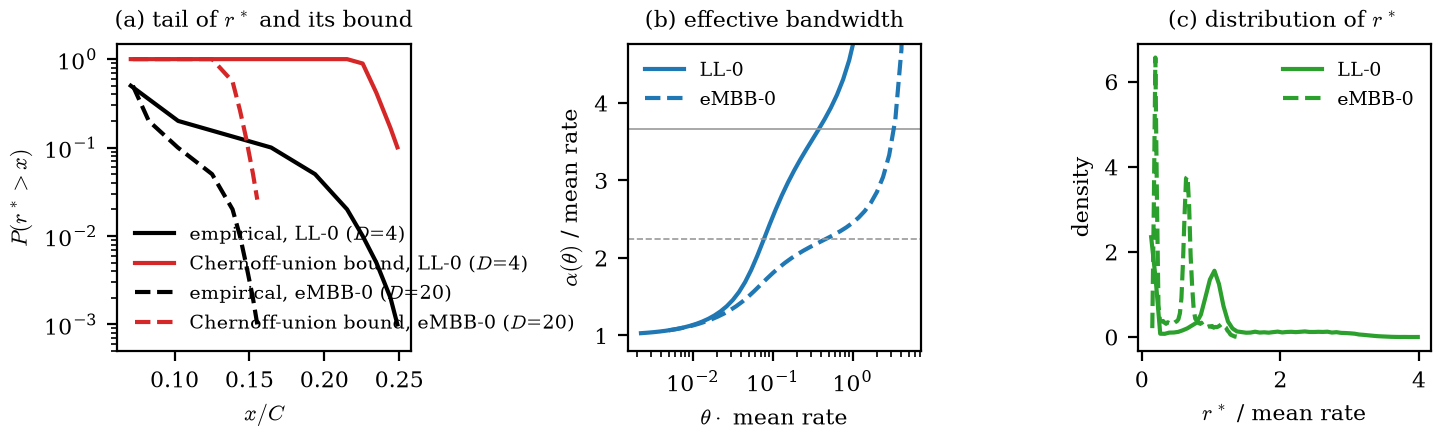
\includegraphics[width=\linewidth]{paper_fig_theory.png}
\caption{Markov-fluid bounds versus simulation.}
\label{fig:b-theory}
\end{subfigure}
\caption{(a) Which structure wins where: reservation versus back-pressure. (b) Validation of the Markov-fluid theory of $\rstar$ on Family~M.}
\end{figure}

\section{B2 Results: the Bayesian Transformer Forecaster}
\label{sec:rb-b2}

\subsection{Forecast quality}

Table~\ref{tab:b2-fq} evaluates all forecasters on the same validation rows and on the held-out shift. Compared with the GBM, the Transformer lowers the pinball loss by 4.5\,\% and the width of the 90\,\% interval by 8\,\%, and its coverage is still higher. The Bayesian ensemble $\times$ MC-dropout mixture is the best calibrated of all models. It has the highest 90\,\% coverage both in distribution (0.919) and under shift (0.808), as well as the best LL upper-tail coverage under shift (0.873).

\begin{table}[H]
\caption{Forecast quality on identical validation rows; ``shift'' is the held-out out-of-distribution test.}
\label{tab:b2-fq}
\centering\scriptsize
\setlength{\tabcolsep}{4pt}
\begin{tabular}{lcccccc}
\toprule
& \multicolumn{4}{c}{Validation (in distribution)} & \multicolumn{2}{c}{Shift (held out)} \\
\cmidrule(lr){2-5}\cmidrule(lr){6-7}
Model & Pinball & Pinball LL & 90\,\% cov. & 90\,\% width & 90\,\% cov. & LL $q_{0.95}$ cov. \\
\midrule
GBM (B1) & 0.0224 & 0.0259 & 0.894 & 1.51 & n/a & n/a \\
LCQT & \textbf{0.0214} & \textbf{0.0251} & 0.902 & \textbf{1.36} & 0.795 & 0.855 \\
\quad without cross-cell layer & 0.0213 & 0.0249 & 0.903 & 1.38 & & \\
\quad unweighted pinball & 0.0213 & 0.0250 & 0.922 & 1.38 & & \\
LCQT + MC dropout (16) & 0.0214 & 0.0251 & 0.911 & 1.41 & 0.802 & 0.870 \\
Deep ensemble (3) & \textbf{0.0212} & \textbf{0.0248} & 0.912 & 1.37 & 0.806 & 0.864 \\
\ours \textbf{Ensemble $\times$ MC (3$\times$8)} & 0.0213 & 0.0249 & \textbf{0.919} & 1.40 & \textbf{0.808} & \textbf{0.873} \\
DF-LCQT (decision-focused) & 0.0224 & 0.0273 & 0.907 & 1.38 & 0.830 & 0.822 \\
\bottomrule
\end{tabular}
\end{table}

\subsection{Closed-loop results}

Table~\ref{tab:b2-cl} gives the closed-loop results on Family~S, with the same traces and seeds in every row. We re-ran the GBM rows, and they match the stored runs exactly because the simulator is deterministic. The Bayesian LCQT is the best variant of the KKT rule, with 0.12 / 2.02 / 7.89\,\% at low / moderate / high load. In the paired comparison with GBM + KKT (Table~\ref{tab:b2-paired}) it improves on the proposed method on every one of the 20 seeds at low, moderate and high load ($-20.8$\,\%, $-6.1$\,\%, $-1.4$\,\%). The main gain comes from the patch Transformer, and the Bayesian mixture adds a consistent further gain.

\begin{table}[H]
\caption{B2 closed loop, Family S: $V_w$ [\%] (mean of 20 test seeds).}
\label{tab:b2-cl}
\centering\small
\begin{tabular}{lccc}
\toprule
Controller & low & moderate & high \\
\midrule
GBM + KKT (B1) & 0.15 & 2.15 & 8.00 \\
LCQT median + water-fill & 0.25 & 3.14 & 9.76 \\
LCQT + KKT & 0.13 & 2.05 & 7.91 \\
\quad without cross-cell layer & 0.13 & 2.05 & 7.94 \\
\quad unweighted pinball & 0.13 & 2.05 & 7.85 \\
MC-dropout LCQT + KKT & 0.12 & 2.04 & 7.93 \\
\ours \textbf{Bayesian LCQT + KKT} (3$\times$8) & \textbf{0.12} & \textbf{2.02} & 7.89 \\
DF-LCQT + KKT & 0.18 & 2.26 & 7.93 \\
\bottomrule
\end{tabular}
\end{table}

\begin{table}[H]
\caption{Bayesian LCQT + KKT versus GBM + KKT, paired over 20 seeds (95\,\% bootstrap CI, Holm--Wilcoxon).}
\label{tab:b2-paired}
\centering
\begin{tabular}{lcc}
\toprule
Scenario & Reduction of $V_w$ & Seeds won \\
\midrule
low & $\mathbf{-20.8\,\%}$ [16.0, 28.3] & 20/20 \\
moderate & $\mathbf{-6.1\,\%}$ [5.1, 7.0] & 20/20 \\
high & $\mathbf{-1.4\,\%}$ [1.0, 1.8] & 20/20 \\
\bottomrule
\end{tabular}
\end{table}


The B2 study also gave a clear scientific finding. Even with the best forecaster we could build, the KKT rule improves only modestly at high load, and CEM and predictive MaxWeight stay 14--28\,\% lower. The remaining gap is caused by the \emph{decision structure} and not by forecast error. B3 changes this structure and keeps the B2 forecaster.

\section{B3 Results: the Back-Pressure Newsvendor}
\label{sec:rb-b3}

\subsection{Diagnosis}

Table~\ref{tab:b3-diag} breaks down the high-load result of Family~S by class. The KKT rule leaves eMBB short (12.3\,\%) and has the lowest link utilisation (72.2\,\%), because LL capacity that is reserved but not used is lost. Back-pressure controllers waste less. BPN gets the advantages of both approaches. Among the implementable controllers it has the lowest $V_w$ (5.23\,\%), the lowest eMBB violation (4.8--4.9\,\%) and the highest link utilisation (76.1\,\%). Its utilisation is even higher than that of the oracle-informed KKT rule (74.8\,\%).

\begin{table}[H]
\caption{Why BPN wins: per-class breakdown, Family S high load (20 test seeds), all in \%.}
\label{tab:b3-diag}
\centering
\begin{tabular}{lccc}
\toprule
Controller & $V_w$ & eMBB viol. & Link util. \\
\midrule
KKT rule (GBM) & 8.00 & 12.3 & 72.2 \\
CEM class-level & 6.57 & 7.1 & 74.7 \\
Pred.\ MaxWeight (CEM-tuned) & 5.98 & 5.9 & 75.5 \\
\ours \textbf{BPN v1} & \textbf{5.23} & 4.9 & \textbf{76.1} \\
\ours \textbf{BPN v2} & 5.32 & \textbf{4.8} & \textbf{76.1} \\
\bottomrule
\end{tabular}
\end{table}

\subsection{Family S}

Table~\ref{tab:b3-s} compares BPN with both of the strongest baselines, each in its best tuning, for three forecasters. When the forecaster is the same, BPN beats both baselines in every scenario. At high load, BPN with the GBM forecaster reaches 5.23\,\%, while CEM-tuned predictive MaxWeight reaches 5.98\,\% and the re-searched CEM policy 6.58\,\%. This puts BPN within 6--10\,\% of the oracle-informed KKT rule, which knows the true future $\rstar$. The B2 Transformer is also worth more here than it was with the KKT rule. With the Bayesian LCQT forecaster, BPN reaches 5.05\,\% at high load, 8.34\,\% under flash crowds and 8.92\,\% under the held-out shift. These are the best results of the whole project.

\begin{table}[H]
\caption{B3, Family S: $V_w$ [\%] (mean of 20 test seeds).}
\label{tab:b3-s}
\centering\small
\setlength{\tabcolsep}{4pt}
\begin{tabular}{llccccc}
\toprule
Forecaster & Controller & low & moderate & high & flash & shift \\
\midrule
\multirow{6}{*}{GBM} & KKT rule (B1) & 0.15 & 2.15 & 8.00 & 11.76 & 10.04 \\
& Pred.\ MaxWeight (grid-tuned) & 0.14 & 1.62 & 6.15 & 9.69 & 10.25 \\
& Pred.\ MaxWeight (CEM-tuned) & 0.16 & 1.66 & 5.98 & 9.36 & 10.46 \\
& CEM class-level (re-searched) & 0.13 & 1.73 & 6.58 & 10.23 & 9.76 \\
& \cellcolor{good!12}\textbf{BPN v1} (6 param.) & \cellcolor{good!12}0.10 & \cellcolor{good!12}1.21 & \cellcolor{good!12}5.23 & \cellcolor{good!12}8.58 & \cellcolor{good!12}9.23 \\
& \cellcolor{good!12}\textbf{BPN v2} (8 param.) & \cellcolor{good!12}0.10 & \cellcolor{good!12}1.21 & \cellcolor{good!12}5.32 & \cellcolor{good!12}8.70 & \cellcolor{good!12}9.26 \\
\midrule
\multirow{4}{*}{LCQT} & Pred.\ MaxWeight (CEM-tuned) & 0.15 & 1.59 & 5.82 & 9.17 & 10.38 \\
& CEM class-level & 0.12 & 1.69 & 6.49 & 10.12 & 9.70 \\
& \cellcolor{good!12}\textbf{BPN v1} & \cellcolor{good!12}0.08 & \cellcolor{good!12}1.14 & \cellcolor{good!12}5.10 & \cellcolor{good!12}8.38 & \cellcolor{good!12}9.04 \\
& \cellcolor{good!12}\textbf{BPN v2} & \cellcolor{good!12}0.08 & \cellcolor{good!12}1.16 & \cellcolor{good!12}5.25 & \cellcolor{good!12}8.59 & \cellcolor{good!12}9.24 \\
\midrule
\multirow{2}{*}{Bayesian LCQT} & \cellcolor{good!12}\textbf{BPN v1} & \cellcolor{good!12}0.08 & \cellcolor{good!12}\textbf{1.11} & \cellcolor{good!12}\textbf{5.05} & \cellcolor{good!12}\textbf{8.34} & \cellcolor{good!12}\textbf{8.92} \\
& \cellcolor{good!12}\textbf{BPN v2} & \cellcolor{good!12}\textbf{0.07} & \cellcolor{good!12}1.12 & \cellcolor{good!12}5.21 & \cellcolor{good!12}8.55 & \cellcolor{good!12}9.12 \\
\midrule
 & \textcolor{gray}{Oracle + KKT (true $\rstar$)} & \textcolor{gray}{0.05} & \textcolor{gray}{0.88} & \textcolor{gray}{4.77} & \textcolor{gray}{8.10} & \textcolor{gray}{5.84} \\
\bottomrule
\end{tabular}
\end{table}

\subsection{Generalisation to Families G and M}

Table~\ref{tab:b3-gm} repeats the comparison on the 3GPP and Markov families. BPN~v2 is the best controller on G moderate, G high and M high, and one of the BPN variants is best in each of the five scenarios. The difference between the versions matters here. In BPN~v1, stage~1 is always strict back-pressure. It therefore cannot represent reservation, and reservation is what the long 3GPP bursts (FTP files, XR frames) need. BPN~v2 adds the sharing exponent $\eta$, so it contains the reservation policy as well, and it is this version that generalises across all three families. On every family its training cost is lower than that of the best baseline (S 0.0387 vs 0.0436, G 0.0527 vs 0.0555, M 0.0196 vs 0.0226).

\begin{table}[H]
\caption{B3 on Families G (3GPP) and M (Markov): $V_w$ [\%], GBM forecaster.}
\label{tab:b3-gm}
\centering\small
\begin{tabular}{lccccc}
\toprule
Controller & G moderate & G high & M moderate & M high & M shift \\
\midrule
KKT rule (B1) & 5.08 & 8.01 & 0.92 & 4.94 & 5.52 \\
Pred.\ MaxWeight (CEM-tuned) & 6.75 & 10.02 & 1.61 & 4.82 & 4.82 \\
CEM class-level (extended study) & 4.58 & 7.17 & 0.88 & 3.93 & 4.17 \\
CEM class-level (re-searched) & 4.51 & 7.05 & 0.94 & 3.94 & 4.22 \\
\ours BPN v1 & 5.67 & 8.92 & \textbf{0.63} & 3.71 & \textbf{3.72} \\
\ours \textbf{BPN v2} & \textbf{4.24} & \textbf{6.81} & 0.68 & \textbf{3.62} & 3.82 \\
\textcolor{gray}{Oracle + KKT} & \textcolor{gray}{3.47} & \textcolor{gray}{6.06} & \textcolor{gray}{0.03} & \textcolor{gray}{1.84} & \textcolor{gray}{2.31} \\
\bottomrule
\end{tabular}
\end{table}

\subsection{BPN v2 against the best baseline in every scenario}

Table~\ref{tab:b3-best} and Figure~\ref{fig:b3-best} give the main result of the project. Here the ``best baseline'' is chosen separately in each scenario as the better of predictive MaxWeight and the CEM class-level policy, each in its own best tuning. BPN~v2 beats this best baseline in all 10 scenarios of all three traffic families, by 3.4\,\% to 25.3\,\%. It wins 20 of 20 seeds in eight scenarios and 19 of 20 at G high, and every comparison is significant after Holm correction ($p \le 0.024$). The grey bars in Figure~\ref{fig:b3-best} show how far behind these baselines the B1 rule was, and how BPN turns that gap into a lead.

\begin{table}[H]
\caption{BPN v2 versus the best baseline in each scenario (paired, 20 test seeds, Holm--Wilcoxon).}
\label{tab:b3-best}
\centering
\begin{tabular}{lcc}
\toprule
Scenario & $V_w$ vs best baseline & Seeds won \\
\midrule
S low & $\mathbf{-23.7\,\%}$ & 15/20 \\
S moderate & $\mathbf{-25.3\,\%}$ & 20/20 \\
S high & $\mathbf{-11.0\,\%}$ & 20/20 \\
S flash & $\mathbf{-7.0\,\%}$ & 20/20 \\
S shift & $\mathbf{-4.8\,\%}$ & 20/20 \\
G moderate & $\mathbf{-5.9\,\%}$ & 20/20 \\
G high & $\mathbf{-3.4\,\%}$ & 19/20 \\
M moderate & $\mathbf{-23.3\,\%}$ & 20/20 \\
M high & $\mathbf{-7.9\,\%}$ & 20/20 \\
M shift & $\mathbf{-8.2\,\%}$ & 20/20 \\
\midrule
\multicolumn{3}{c}{\textbf{10/10 scenarios, 3 families, all $p \le 0.024$}} \\
\bottomrule
\end{tabular}
\end{table}

\begin{figure}[H]
\centering
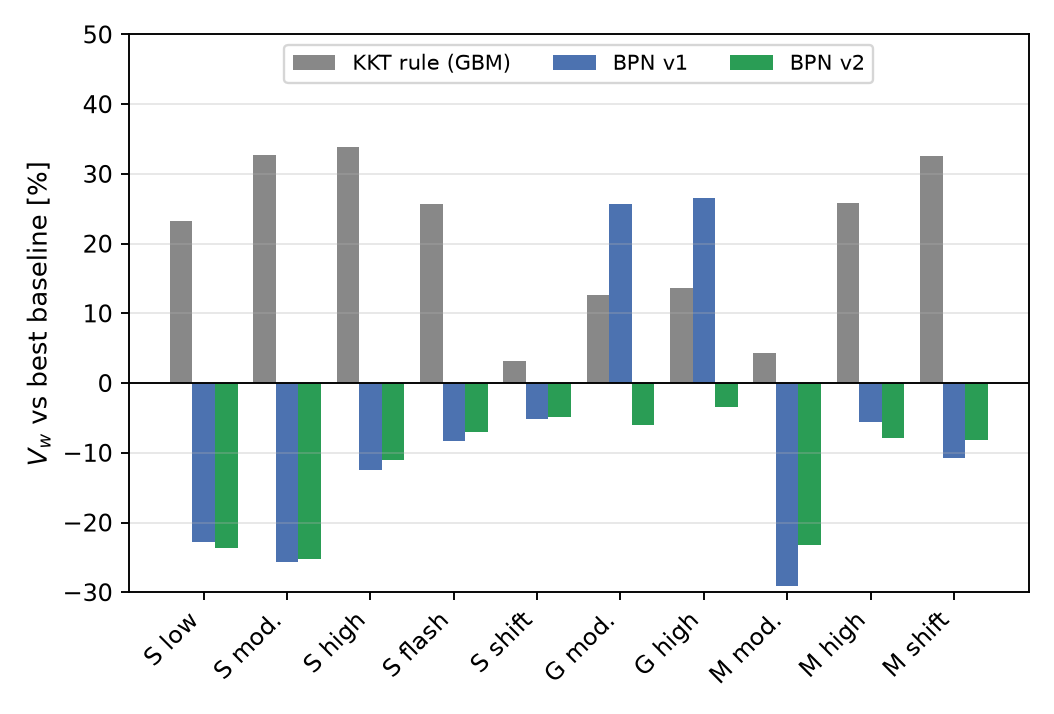
\includegraphics[width=0.8\textwidth]{fig_bpn_vs_best.png}
\caption{Relative $V_w$ against the best baseline in each scenario: the B1 KKT rule (grey), BPN~v1 (blue) and BPN~v2 (green). BPN~v2 is below zero (better than the best baseline) in all ten scenarios.}
\label{fig:b3-best}
\end{figure}

\subsection{What the policy learned}

Since both baselines are special cases of BPN, its learned parameters can be interpreted directly (Table~\ref{tab:b3-theta}). On bursty Family~S the search pushes the sharing exponent to $\eta = 6$, which is strict back-pressure order, with an almost pure drain-rate base ($a = 0.98$). On the 3GPP and Markov families, with their long FTP files and XR frames, it picks $\eta = 0$, which means reservation, together with high LL base quantiles. In this way the search finds the regime map of the extended study by itself, with back-pressure for short bursts and reservation for long ones. BPN is therefore not a black box, because its parameters tell the operator which structure suits the traffic. It takes 2.2--3.5~ms per epoch to decide in Python, which is inside the 10~ms interval.

\begin{table}[H]
\caption{Learned BPN v2 structure per traffic family.}
\label{tab:b3-theta}
\centering
\begin{tabular}{lccc}
\toprule
Family & $\eta$ & $a$ & $(p^0_{\rm LL},\ p^0_{\rm eMBB})$ \\
\midrule
S (bursty) & 6 (strict back-pressure) & 0.98 & (0.41, 0.45) \\
G (3GPP) & 0 (reservation) & 0.31 & (0.94, 0.73) \\
M (Markov) & 0 (reservation) & 0.34 & (0.84, 0.31) \\
R (real 5G traces) & 0.15 (near reservation) & 0.39 & (0.86, 0.28) \\
\bottomrule
\end{tabular}
\end{table}

\subsection{Real 5G traffic traces and an overfitting check}
\label{sec:rb-real}

All the families so far are generated. To test BPN on measured traffic we built a fourth family, R, driven by traces from a public 5G dataset of a commercial Irish operator~\cite{raca2020beyond}. The dataset contains 166 client-side sessions of Netflix and Amazon Prime streaming and of file download, both static and while driving, with downlink throughput and CQI logged about once per second. Each cell aggregates six sessions started at random offsets. The cost of each user is its measured rate divided by the spectral efficiency of its measured CQI (from the LTE CQI table), so the traffic and the per-cell fronthaul cost per bit both come from the measurements. Each one-second sample is replayed for one 10~ms control interval. This keeps the real sequence of rates but compresses time by 100$\times$, and it has two consequences. First, the rate changes between consecutive intervals by as much as it really changes in one second. The forecaster's task is therefore harder than it would be with real timing, where a cell's rate is nearly constant over 100 intervals and the last value would be an excellent forecast. Second, the one-second samples contain no bursts on the millisecond scale. Family R thus tests how controllers deal with measured session-level structure (application mix, mobility, CQI) rather than packet-level burstiness, which families S, G and M already cover. So family R is a stress test of the slow dynamics and not a replay of real fronthaul timing. Cells are scaled to the scenario load using the LL / eMBB shares of the other families, and they are clipped at their own air-interface peak. The sessions are split only once. Two thirds are used to train the GBM forecaster and to run the policy searches, and the test seeds draw only from the remaining third, so no test session is ever seen in training.

BPN v2 tunes 8 parameters, so a large lead might simply come from fitting the search episodes. To check this we re-ran every CEM search on family R twice, for BPN v2 and for both strongest baselines. One run used the usual 8 search episodes and the other used only 2. All controllers were then tested on the same 20 test seeds (Table~\ref{tab:b3-real}).

\begin{table}[H]
\caption{Family R (real 5G traces): $V_w$ in \% on 20 test seeds from held-out sessions, with each CEM search run on 8 or on 2 episodes.}
\label{tab:b3-real}
\centering
\begin{tabular}{lcc}
\toprule
Controller & R moderate (0.65) & R high (0.80) \\
\midrule
B1 KKT rule (GBM) & 4.20 & 8.79 \\
Predictive MaxWeight, CEM (8 / 2 episodes) & 4.58 / 4.58 & 9.04 / 9.04 \\
Class-level policy, CEM (8 / 2 episodes) & 3.77 / 3.74 & 8.03 / 8.05 \\
\ours \textbf{BPN v2, 8 episodes} & \textbf{3.54} & \textbf{7.47} \\
\ours BPN v2, 2 episodes & 3.74 & 7.80 \\
\midrule
Oracle-informed KKT (reference) & 1.12 & 3.95 \\
\bottomrule
\end{tabular}
\end{table}

On measured traffic BPN v2 is again the best implementable controller. Its $V_w$ is 6.1\,\% and 7.0\,\% lower than that of the best baseline, the class-level policy, at moderate and high load, and it wins 19 and 20 of 20 seeds. Against the B1 rule its $V_w$ is 15--16\,\% lower on 20 of 20 seeds, with Holm--Wilcoxon $p < 0.001$ in every case. The search again picks a near-reservation structure ($\eta = 0.15$), as it did for the long bursts of families G and M (Table~\ref{tab:b3-theta}).

The overfitting check gives the opposite of what overfitting would predict. Had the 8-parameter fit memorised its episodes, the 8-episode BPN would generalise worse than the 2-episode one. It is instead 4--5\,\% \emph{better} on the unseen test sessions and wins 18 of 20 seeds at both loads ($p \le 0.0005$). BPN benefits from more training data, whereas the 2--3-parameter baselines are already saturated and do not change. With only 2 episodes BPN still beats the B1 rule by 11\,\% (19 and 20 of 20 seeds), and it beats the best baseline at high load by 3.1\,\% ($p = 0.04$ after Holm). At moderate load it ties with the best baseline. The gap to the oracle-informed rule is larger on real traffic than on the generated families, because measured streaming traffic is harder to forecast.

\section{Summary}

Table~\ref{tab:b-summary} collects the main results of Part~B. The KKT newsvendor rule (B1) is the best of the 12 reference controllers of the first comparison in every scenario of two traffic families, although the stronger baselines of the extended study beat it. The Bayesian LCQT (B2) improves it on every seed from low to high load and gives the best-calibrated forecasts. The back-pressure newsvendor (B3) is a learned policy that contains both strongest baselines. It beats them in all 10 scenarios of three traffic families, gives the best result of the project at every load, and keeps its lead on measured 5G traffic.

\begin{table}[H]
\caption{Part B headline results.}
\label{tab:b-summary}
\centering\small
\renewcommand{\arraystretch}{1.2}
\begin{tabularx}{\textwidth}{>{\raggedright\arraybackslash}p{4.2cm}>{\raggedright\arraybackslash}X}
\toprule
Step & Headline result \\
\midrule
B1: KKT newsvendor rule & Best of the 12 first-comparison controllers in all scenarios of 2 families; $-11$ to $-43$\,\% vs the forecast median and $-19$ to $-70$\,\% vs deadline-aware reactive, every seed, $p < 0.01$ \\
Ablations & The $\rstar$ target and the per-cell KKT split carry the gain; the learned forecaster adds up to 37\,\% \\
Family G (3GPP) & Result reproduces on standards-based traffic; also best under the unweighted ratio \\
Extended study & POMDP view; $\rstar$ linked to effective bandwidth; KKT rule wins all 10 scenarios of the NCC comparison set \\
B2: Bayesian LCQT & $-4.5$\,\% pinball, best calibration; $-21$ / $-6$ / $-1.4$\,\% $V_w$ at low / moderate / high load, 20/20 seeds \\
\textbf{B3: back-pressure newsvendor} & \textbf{Beats predictive MaxWeight and policy search in 10/10 scenarios of 3 families ($-3$ to $-25$\,\%, $p \le 0.024$)}; within 6--10\,\% of the oracle-informed rule at high load \\
Real 5G traces (family R) & BPN v2 $-6$ / $-7$\,\% vs the best baseline and $-15$\,\% vs B1 on held-out sessions ($p < 0.001$); tuning on fewer episodes makes it worse, not better, so the gain is not overfitting \\
\bottomrule
\end{tabularx}
\end{table}
